\documentclass{beamer}
\usepackage[italian]{babel}
\usetheme{Berkeley}
\usepackage{graphicx}
\usepackage{booktabs}
\graphicspath{{figures/}}

\title{Condividere informazioni in modo \\
sicuro combinando Git e Blockchain}
\author{Paolo Speziali}
\institute{Università degli Studi di Perugia - Dipartimento di Ingegneria\\[\medskipamount]
      
\includegraphics[width=0.35\textwidth]{figures/logo_unipg.png}
 }
\logo{
\includegraphics[height=1cm]{favicon.png}}
\date{A.A. 2020/2021}

\begin{document}
\begin{frame}
	\titlepage % beamer's \maketitle
\end{frame}
\begin{frame}
	\frametitle{Indice}
	\tableofcontents
\end{frame}
\section{Introduzione}
\begin{frame}
	\frametitle{La digitalizzazione}
	È in atto, negli ultimi anni, un piano di \textbf{digitalizzazione} delle PA.
	Esso mira all'evoluzione tecnologica di tutte le sue mansioni e alla creazione
	di portali web per il cittadino.
	L'esigenza di questa trasformazione si è fatta sentire anche da parte
	dell'Unione Europea, che con il Recovery Fund
	ci sta fornendo i fondi per attuarla.
	\begin{figure}
		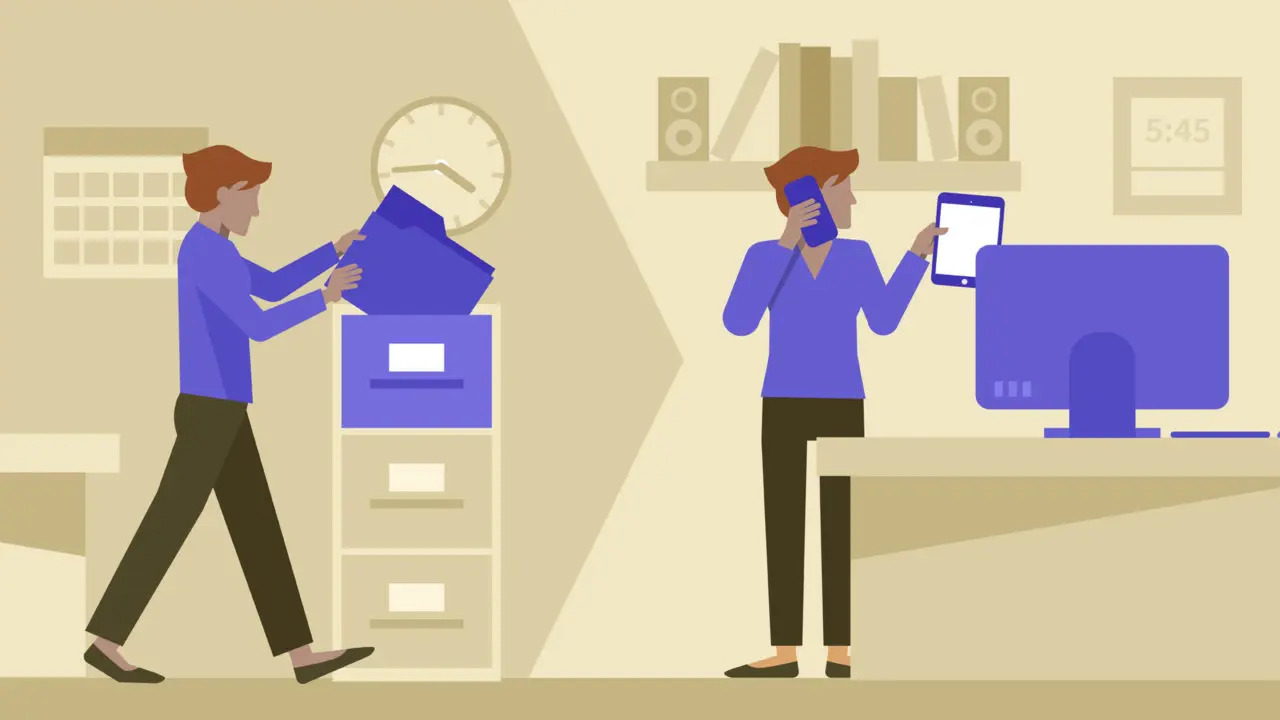
\includegraphics[width=0.55\textwidth]{digitalizzazione.jpg}
		% https://www.agendadigitale.eu/documenti/digitalizzazione-della-pa-in-italia-la-strategia-delle-tre-c/
	\end{figure}
\end{frame}

\begin{frame}
	\frametitle{Il problema della burocrazia}
	Tuttavia, anche avendo i fondi necessari, sono molti i problemi che non permettono
	una digitalizzazione totale delle PA, tra cui la lenta e farraginosa macchina
	della burocrazia. Sembra necessario un processo di \textbf{sburocratizzazione}
	grazie a degli strumenti digitali che permettano di salvare,
	validare e condividere documenti in maniera sicura.
	\medskip
	\begin{figure}
		
\includegraphics[width=0.65\textwidth]{buro.jpg}
		% https://www.identitafutura.it/burocrazia-allitaliana/
	\end{figure}
\end{frame}

\begin{frame}
	\frametitle{Gli strumenti attuali}
	\begin{columns}
		\column{0.5\textwidth}
		Gli strumenti attualmente in utilizzo hanno un'architettura centralizzata:
		un'entità centrale si occupa dell'immagazzinamento e della verifica dei dati
		degli utenti. Ciò è potenzialmente rischioso, sia perché potrebbero verificarsi
		attacchi alle unità centrali,
		sia perché mettiamo in mano di un'azienda esterna i nostri dati.
		\column{0.5\textwidth}
		\begin{figure}
			
\includegraphics[width=0.80\textwidth]{cent.png}
			% https://icon-icons.com/it/icona/centralizzato-rete-dati-blockchain-tecnologia/95906
		\end{figure}
	\end{columns}
\end{frame}

\begin{frame}
	\frametitle{Strumenti decentralizzati}
		Usando invece strumenti decentralizzati, sia per la gestione dei file,
		per cui utilizzeremo \textbf{Git}, sia per la verifica delle informazioni,
		per cui useremo la \textbf{blockchain}, saremo in grado costruire uno strumento
		che può affidarsi alla parola di una moltitudine di entità, rendendo molto
		più complicati e rilevabili attacchi e manomissioni.
	\medskip
	\begin{figure}
		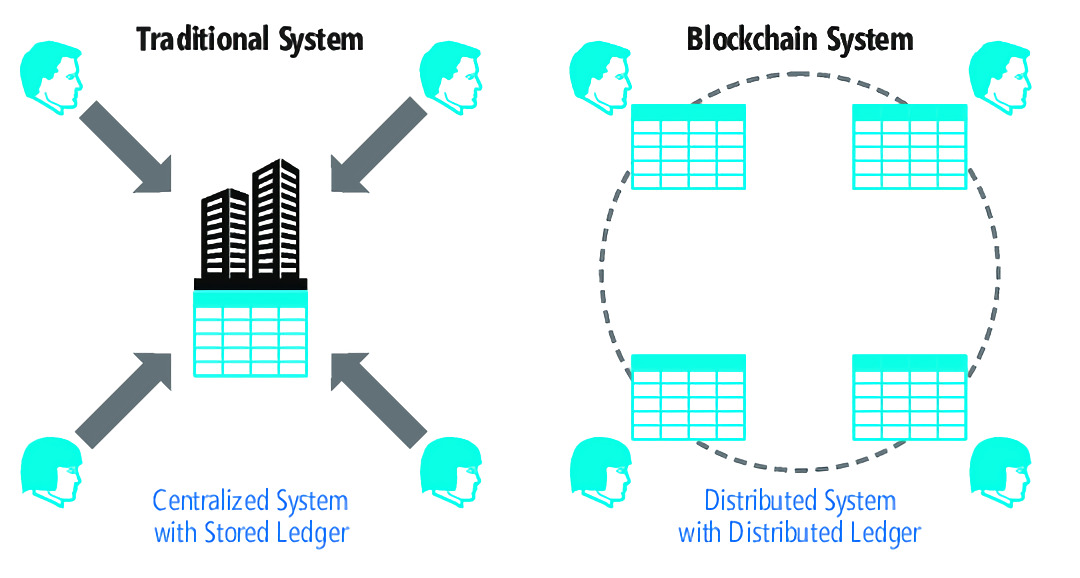
\includegraphics[width=0.70\textwidth]{dece.jpg}
		% https://docs.microsoft.com/it-it/archive/msdn-magazine/2018/july/blockchain-decentralized-applications-with-azure-blockchain-as-a-service
	\end{figure}
\end{frame}

\section{Concetti preliminari}
\begin{frame}
	\frametitle{Funzioni crittografiche di hashing}
	Una funzione crittografica di hashing è una funzione di hashing, ovvero
	una funzione che permette di associare,
	a una qualsiasi sequenza \(m\) di lunghezza arbitraria in input, una sequenza
	in output \(h(m)\) di lunghezza costante,
	con alcune proprietà aggiunte che deve seguire per poter essere considerata
	\emph{crittograficamente sicura}. Esse impediscono di risalire all'input originale
	e facilitano i \textbf{controlli di integrità sui file}.
	\medskip
	\begin{figure}
		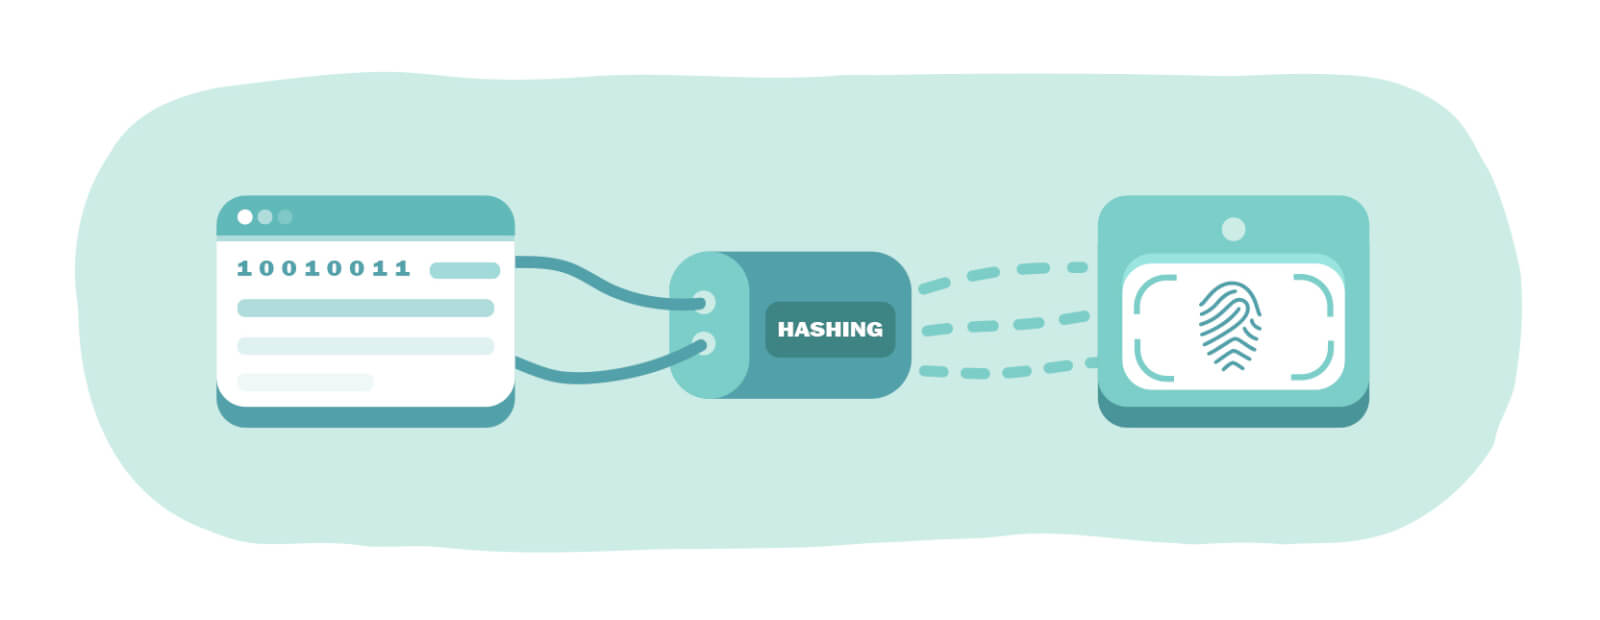
\includegraphics[width=0.85\textwidth]{figures/hashing.jpg}
	\end{figure}
\end{frame}

\section{Il Problema e l'Obiettivo}
\begin{frame}
	\frametitle{Il Problema}
	Una funzione crittografica di hashing è una funzione di hashing, ovvero
	una funzione che permette di associare,
	a una qualsiasi sequenza \(m\) di lunghezza arbitraria in input, una sequenza
	in output \(h(m)\) di lunghezza costante,
	con alcune proprietà aggiunte che deve seguire per poter essere considerata
	\emph{crittograficamente sicura}. Esse impediscono di risalire all'input originale
	e facilitano i \textbf{controlli di integrità sui file}.
	\medskip
	\begin{figure}
		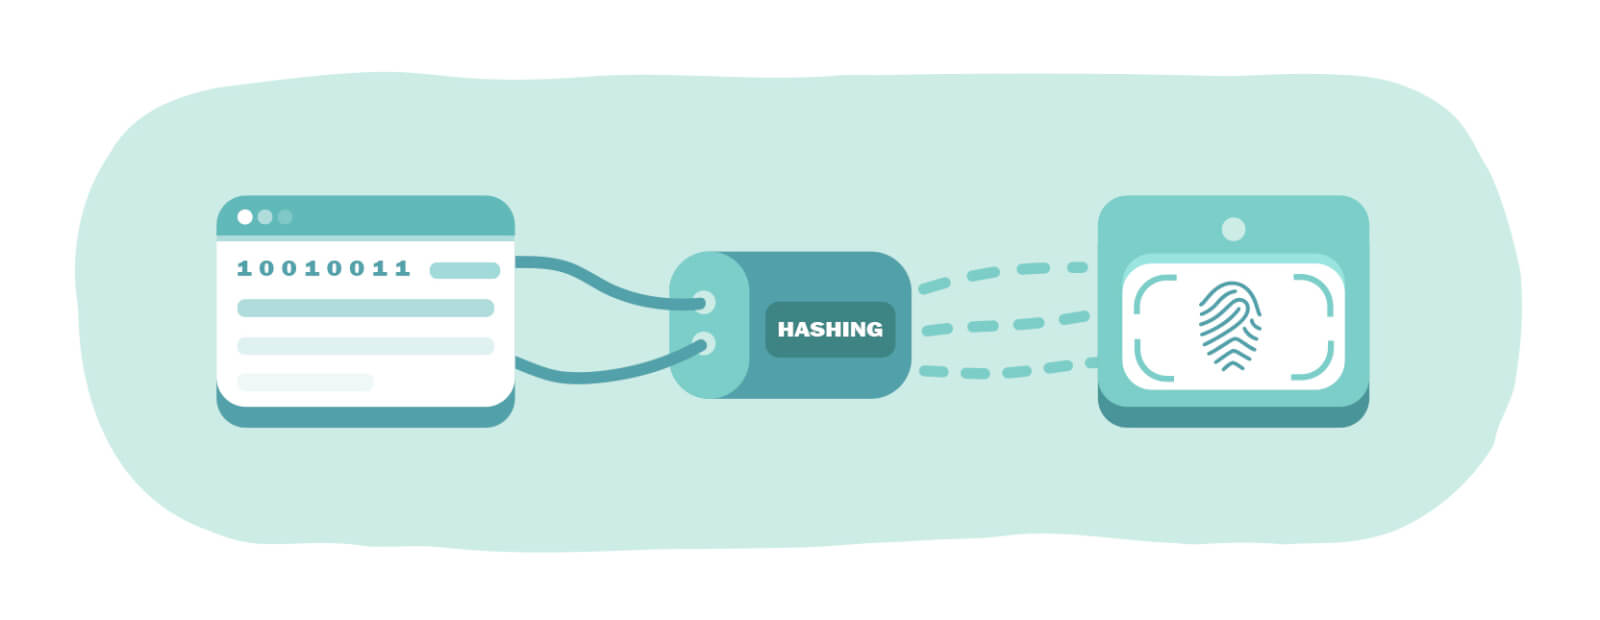
\includegraphics[width=0.85\textwidth]{figures/hashing.jpg}
	\end{figure}
\end{frame}


\begin{frame}
	\frametitle{Fase 2: Specifica dei requisiti}
	\begin{columns}
		\column{0.5\textwidth}
		L'applicazione avrebbe dovuto quindi fornire all'utilizzatore le funzionalità del software Git corredando il tutto con la possibilità di registrare e, successivamente, verificare l'integrità delle Storage Unit. Una volta creata una Storage Unit essa deve essere immutabile, dando tuttavia la possibilità di esportarne singoli file dotandoli sempre di meccanismi di controllo.
		\column{0.5\textwidth}
		\begin{figure}
			
\includegraphics[width=0.55\textwidth]{figures/favicon.png}
			\caption{Il logo dell'applicazione}
		\end{figure}
	\end{columns}
\end{frame}

\begin{frame}
	\frametitle{Excursus su Ethereum e Blockchain}
	La tecnologia di Ethereum permette la creazione di una rete distribuita e decentralizzata finanziata e incentivata ad operare e rimanere attiva mediante la creazione, lo scambio e l’utilizzo dell’omonima criptovaluta.
	\medskip
	\begin{figure}
		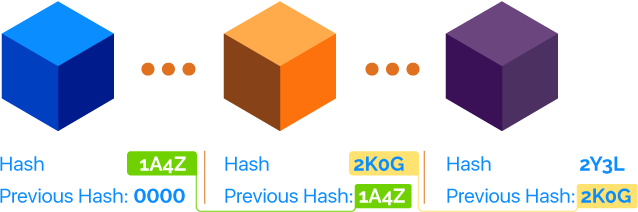
\includegraphics[width=0.60\textwidth]{figures/blockchain.png}
	\end{figure}
\end{frame}
\begin{frame}
	\frametitle{Excursus sulle Applicazioni Distribuite}
	\begin{figure}
		
\includegraphics[width=0.90\textwidth]{figures/truffle.png}
	\end{figure}
	\bigskip
	Su tale rete è possibile mettere a disposizione delle applicazioni che chiunque può utilizzare dietro pagamento di una piccola commissione. Queste applicazioni sono realizzabili dagli sviluppatori interessati tramite vari framework e suite di applicativi, il più celebre è \textbf{Truffle}.
\end{frame}
\begin{frame}
	\frametitle{Excursus su Git}
	Git è un software che permette in maniera semplice di gestire insiemi di file tramite un sistema di controllo di versione, una grande risorsa per gli sviluppatori che devono contribuire in maniera condivisa ad uno stesso progetto o che devono tenere sotto controllo i vari cambiamenti che sono stati apportati ai vari file e documenti.
	\begin{figure}
		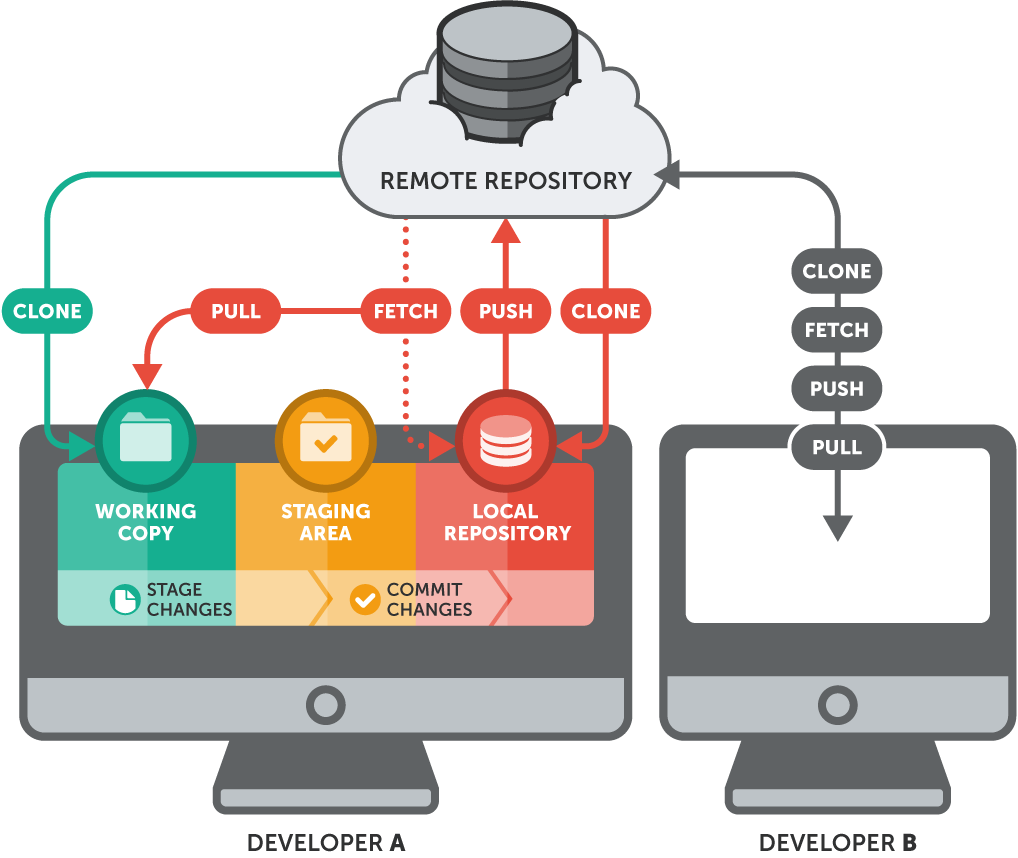
\includegraphics[width=0.45\textwidth]{figures/git2.png}
	\end{figure}
\end{frame}
\begin{frame}
	\frametitle{Excursus sulle funzioni di hashing}
	Le funzioni di hashing sono funzioni non invertibili che permettono di associare in maniera univoca (o quasi) stringhe di caratteri (e quindi anche documenti di varia natura tradotti in stringhe) a delle stringhe alfanumeriche di lunghezza fissa.
	\bigskip
	\begin{figure}
		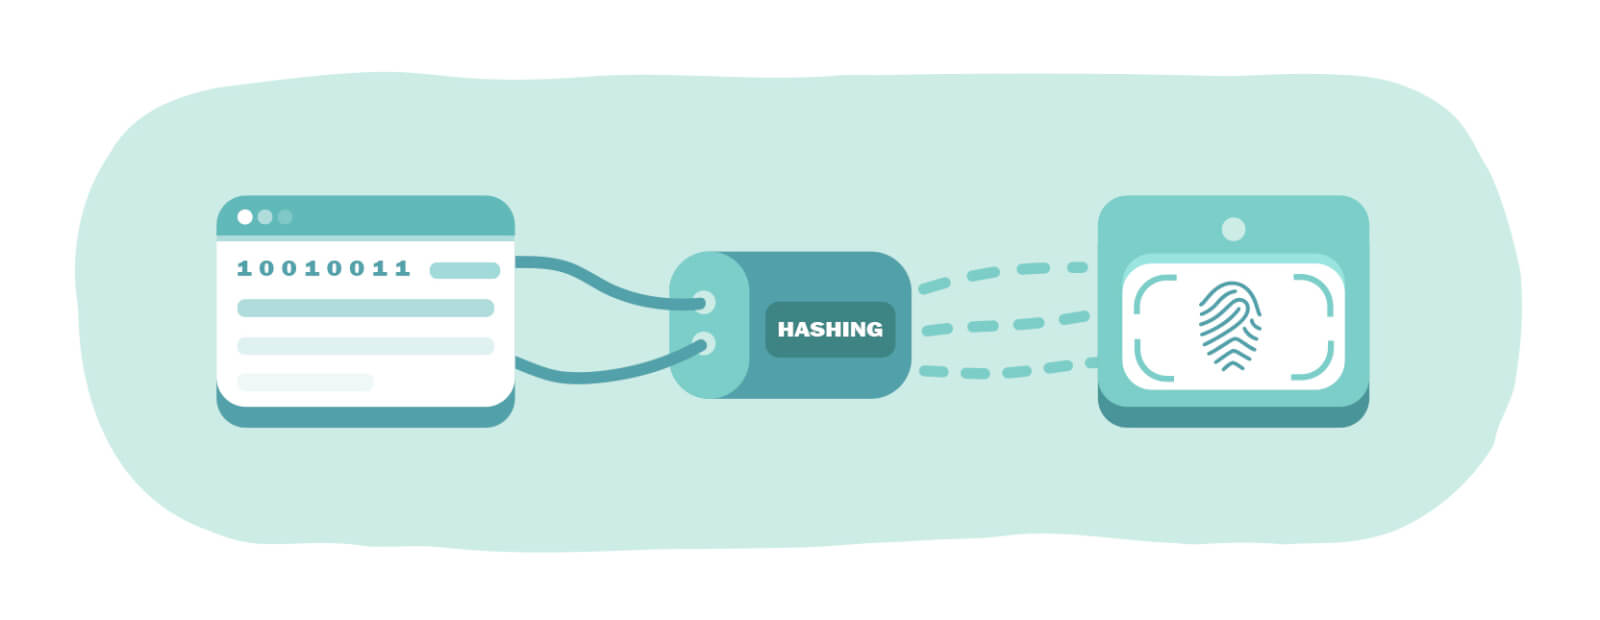
\includegraphics[width=0.85\textwidth]{figures/hashing.jpg}
	\end{figure}
\end{frame}

\section{Fonti}
\begin{frame}
	\frametitle{Fonti}
	\begin{itemize}
		\item \href{https://ethereum.org/it/developers/}{Strumenti Ethereum per sviluppatori} 
  		\item \href{https://www.trufflesuite.com/tutorial}{Tutorial Truffle DAPPs - Pet Shop}
  		\item \href{https://www.sitepoint.com/javascript-command-line-interface-cli-node-js/}{Build a JavaScript CLI with Node.js}
  		\item \href{https://developer.mozilla.org/en-US/docs/Learn/JavaScript/Asynchronous/Async_await}{Tutorial di Mozilla su async / await}
  		\item Immagini reperite dai siti ufficiali degli strumenti eccetto per alcune scaricate da queste pagine web:
			\begin{itemize}
				\item \href{https://www.poeticoding.com/hashing-a-file-in-elixir/}{Funzioni di Hashing}
				\item \href{https://www.romatoday.it/attualita/concorso-rai-fiera-roma-norme-covid-19.html}{Concorso pubblico}
				\item \href{https://www.criptovalute24.com/ethereum-migliora-la-sua-blockchain-rialzo-del-5-4/}{Ethereum Blockchain}
				\item \href{https://blog.netsons.com/git-software-guida-facile/}{Git repository}
				\item \href{https://amerlin.keantex.com/programmazione-asincrona-con-async-await-parte-2/}{async / await}
				\item \href{https://transparency.dev/verifiable-data-structures/}{Merkle Tree}
			\end{itemize}
			\item \href{https://waifu2x.booru.pics/Home/index}{Strumento di upscaling delle immagini} 
	\end{itemize}
\end{frame}
\end{document}